% --- Program Section ---

\newprogram{Program 11}{Implement lengthOfLIS(nums: List[int]) -> int function accepting an integer array and
returning the length of the longest strictly increasing subsequence.}

\subsection*{Code}


\begin{lstlisting}[language=python]
from typing import List
import bisect

def lengthOfLIS(nums: List[int]) -> int:
    dp = []

    for num in nums:
        # Find the first element >= num
        pos = bisect.bisect_left(dp, num)

        if pos == len(dp):
            dp.append(num)
        else:
            dp[pos] = num

    return len(dp)


# Example
nums = [10, 9, 2, 5, 3, 7, 101, 18]

print("Length of LIS:", lengthOfLIS(nums))
\end{lstlisting}

\subsection*{Output}
\begin{center}
    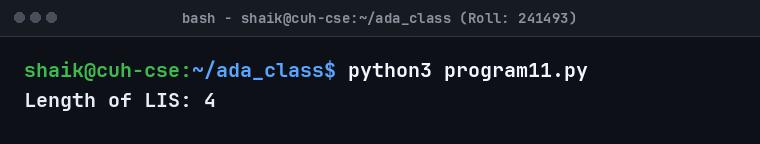
\includegraphics[width=0.88\textwidth]{Images/output_screenshot11.png}
\end{center}

\subsection*{GitHub Scan Code}
\begin{center}
    \begin{minipage}{0.3\textwidth}
        \centering
        % Generates a 2.5cm high QR code directly linking to the code file
        \qrcode[height=3.5cm]{https://github.com/gytdrop/ada_class/blob/main/program11.py} \\[0.2cm]
        \scriptsize\ttfamily Scan to view source code 
    \end{minipage}
\end{center}


% Add a horizontal line that indicates the END of the program.
\vspace{1cm}
\begin{center}
    \rule{1\textwidth}{1pt} % Clean, centered 1pt thick horizontal line
\end{center}